\documentclass{fenicscourse}
% General math notation
\newcommand{\N}{\mathbb{N}}
\newcommand{\PP}{\mathbb{P}}
\newcommand{\QQ}{\mathbb{Q}}

% Math operators
\DeclareMathOperator{\ord}{ord}
\DeclareMathOperator{\Kern}{ker}
\DeclareMathOperator{\Image}{im}
\DeclareMathOperator{\spann}{span}
\DeclareMathOperator{\diam}{diam}


% Mesh and FEM notation
%\newcommand{\dx}{\, \mathrm{d} x}
%\newcommand{\ds}{\, \mathrm{d} s}
%\newcommand{\dS}{\, \mathrm{d} S}
\newcommand{\mesh}{\mathcal{T}}
\newcommand{\facets}{\mathcal{F}}
\newcommand{\inmesh}{\partial_i \mathcal{T}}
\newcommand{\exmesh}{\partial_e \mathcal{T}}

\newcommand{\jump}[1]{\llbracket #1 \rrbracket}
\newcommand{\avg}[1]{\langle #1 \rangle}
\newcommand{\meanvalue}[1]{\langle #1 \rangle}
\newcommand{\vect}[1]{\mathbf{#1}}

\newcommand{\gradhterm}[2]{(\nabla_h #1, \nabla_h #2)_{\Omega}}
\newcommand{\consterm}[2]{(\avg{\nabla_h #1} \dotn,\jump{#2})_{\inmesh}}
\newcommand{\penterm}[2]{( h^{-1} \jump{#1}, \jump{#2})_{\inmesh}}

\newcommand{\Ctr}{C_{\text{tr}}}

% Abbreviations for names etc
\newcommand{\apriori}{\emph{a~priori}}
\newcommand{\aposteriori}{\emph{a~posteriori}}

% Dimensions
\newcommand{\codesize}{\footnotesize}

% Environments
\DefineVerbatimEnvironment{code}{Verbatim}{frame=single,rulecolor=\color{blue}}

% Notes
\newcommand{\amnote}[1]{\todo[inline,color=blue!40]{\underline{AM:} #1}}
\newcommand{\mglnote}[1]{\todo[inline,color=red!40]{\underline{MGL:} #1}}
\newcommand{\alnote}[1]{\todo[inline,color=green!40]{\underline{AL:} #1}}
\newcommand{\mernote}[1]{\todo[inline,color=pink!40]{\underline{MER:} #1}}

% Special notation PI
\newcommand{\OmegaD}{\Omega_{0,\mathrm{D}}}
\newcommand{\OmegaN}{\Omega_{0,\mathrm{N}}}
\newcommand{\OmegaO}{\Omega_{_\mathrm{O}}}
\newcommand{\bfsigma}{{\pmb\sigma}}
\newcommand{\bfepsilon}{{\pmb\epsilon}}

% Special notation for PII
\newcommand{\bfu}{\boldsymbol{u}}
\newcommand{\bff}{\boldsymbol{f}}
\newcommand{\bfg}{\boldsymbol{g}}
\newcommand{\bfv}{\boldsymbol{v}}
\newcommand{\bfe}{\boldsymbol{e}}
\newcommand{\bfn}{\boldsymbol{n}}
\newcommand{\bfx}{\boldsymbol{x}}
\newcommand{\Oast}{\Omega^{\ast}}
\newcommand{\Vast}{\mathcal{V}^{\ast}}

%\newcommand{\meshast}{\mathcal{T}_{\ast}}
\newcommand{\pO}{\partial \Omega}
\newcommand{\meshast}{\mathcal{T}^{\ast}}
\newcommand{\Fast}{\mathcal{F}^{\ast}_{\Gamma}}
\newcommand{\piast}{\pi^{\ast}_h}
\newcommand{\tnast}{\tn_{\ast}}
\newcommand{\tnsip}{\tn_{\text{sip}}}
\newcommand{\tnsipast}{\tn_{\text{sip},\ast}}
\newcommand{\asip}{a^{\text{sip}}_h}

\newcommand{\mcF}{\mathcal{F}}
\newcommand{\mcT}{\mathcal{T}}
\newcommand{\mcV}{\mathcal{V}}
\newcommand{\mcE}{\mathcal{E}}
\newcommand{\mcN}{\mathcal{N}}
\newcommand{\mcC}{\mathcal{C}}
\newcommand{\mcA}{\mathcal{A}}
\newcommand{\tn}{|\mspace{-1mu}|\mspace{-1mu}|}
\newcommand{\Pzero}{P_h^{0,\mathrm{dc}}}
\newcommand{\Pone}{P_h^1}
\newcommand{\ndot}{\bfn \cdot}
\newcommand{\dotn}{\cdot \bfn}
\newcommand{\bfw}{\boldsymbol{w}}
\newcommand{\Wspace}{{\mathcal{V}_h}}

% Special notation for PIII
\newcommand{\nablan}{\partial_{\bfn}}
\newcommand{\OmcupOm}{\Omega_1 \cup \Omega_2}
\newcommand{\mcupm}{{\mathcal{T}^{\ast}_1} \cup \mesh_2}
%\newcommand{\mcupm}{{\meshast}_1 \cup \mesh_2}
%\newcommand{\meanvalue}[1]{\langle #1 \rangle_{\alpha}}
\newcommand{\ifnormalpha}[1]{\ifnorm{#1}{\alpha}}
\newcommand{\ifnorm}[2]{\| #1 \|_{#2,h,\Gamma}}
\newcommand{\tildev}{\widetilde{\bfv}}
\newcommand{\bfphi}{\boldsymbol{\phi}}
\newcommand{\picorr}{\pi^c}

% Math macros
\newcommand{\renni}[2]{\langle #2 ,\; #1 \rangle}


\begin{document}

\fenicslecture{Lecture 8: The Stokes problem}
              {Andr\'e Massing, Kent-Andre Mardal}

%\linespread{1.5}

% Introduction
\begin{frame}
  \frametitle{The Stokes equations}
  \begin{alignat*}{3}
    -\Delta u + \nabla p &= f    &&\quad \text{in } \Omega &&\qquad \text{Momentum equation}\\
          \nabla \cdot u &= 0 \quad &&\quad \text{in } \Omega &&\qquad
    \text{Continuity equation}\\
                       u &= g_D  &&\quad \text{on } \pO_D && \\
    \dfrac{\partial u}{\partial n} -p n &=  g_N &&\quad \text{on } \pO_N&
  \end{alignat*}
  \linespread{1.0}
  \begin{itemize}
    \item
      $u$ is the fluid velocity and $p$ is the pressure
    \item
      $f$ is a given body force per unit volume
    \item
      $g_{_\mathrm{D}}$ is a given boundary flow
    \item
      $g_{_\mathrm{N}}$ is a given function for the natural boundary condition
  \end{itemize}
\end{frame}

%  We consider the stationary Stokes equations: find the velocity $u$
%  and the pressure $p$ such that
%  \begin{equation*}
%    \begin{split}
%      - \Div (\nu \Grad u - p \, \mathrm{I}) &= f \quad \mbox{in } \Omega \\
%      \Div u &= 0 \quad \mbox{in } \Omega \\
%    \end{split}
%  \end{equation*}
%  with boundary conditions
%  \begin{equation*}
%    \begin{split}
%      u &= 0 \quad \mbox{on } \partial \Omega_D \\
%      (\nu \Grad u - p \, \mathrm{I}) \cdot n &= p_0
%      \quad \mbox{on } \partial \Omega_N
%    \end{split}
%  \end{equation*}
%
%  If viscosity $\nu$ varies with $u$ (or $p$),
%  \begin{equation*}
%    \nu = \nu(u)
%  \end{equation*}
%  this is a nonlinear system of partial differential equations.

\begin{frame}
  \frametitle{Variational problem}
  Multiply the momentum equation by a test function $v$ and integrate
  by parts:
  \begin{align*}
    \int_{\Omega} \nabla u : \nabla v \dx
      - \int_{\Omega} p \nabla \cdot
    v \dx
      = \int_{\Omega} f \cdot v \dx + \int_{\pO_N} g_N \cdot
    v \ds
  \end{align*}
  Short-hand notation:
  \begin{equation*}
    \underbrace{
      \inner{\nabla u}{\nabla v}
    }_{a(u,v)}
    \underbrace{
  - \inner{p}{\nabla \cdot v}
  }_{b(v,p)}
    = \underbrace{
   \inner{f}{v} + \inner{g_N}{v}_{\pO_N}
  }_{L(v)}
  \end{equation*}
  Multiply the continuity equation by a test function $q$:
  \begin{equation*}
    \underbrace{\alert{\pm}\inner{\nabla \cdot u}{q}}_{b(u,q)} = 0
  \end{equation*}
  Definitions of $a(\cdot,\cdot)$ and $b(\cdot,\cdot)$ are meaningful if
  $u \in H^1(\Omega)$ and $p \in L^2(\Omega)$

%  Sum up: find $(u, p) \in V$ such that
%  \begin{align*}
%  \inner{\nabla u}{\nabla v}
%  - \inner{p}{\nabla \cdot v}
%  \alert{\pm} \inner{\nabla \cdot u}{q}
%  = \inner{f}{v}  - \inner{ g_N}{v}_{\pO_N}
%  \end{align*}
%  for all $(v, q) \in \hat{V}$
\end{frame}


\begin{frame}
  \frametitle{Saddle point formulation of the Stokes problem}
  The Stokes problem is an example of a \colemph{saddle point
  problem}:
  Find $(u,p) \in V \times Q$
  such that
  for all  $(v,q) \in \widehat{V} \times \widehat{Q}$
  \begin{alignat*}{2}
    &a(u,v) + b(v,p) & &= L(v)
    \\
    &b(u,q) \phantom{a(u,v)} & &= 0
  \end{alignat*}
  Sum up:
  $A(u,p;v,q) := a(u,v) + b(v,p) + b(u,q) = L(v)$
  \\
  \colemph{Mixed spaces}:
  \begin{align*}
    V &=  [H^1_{g_D,\Gamma_D}(\Omega)]^d &\quad  \widehat{V} &=
    [H^1_{0,\Gamma_D}(\Omega)]^d \\
    Q &= L^2(\Omega) &\quad \widehat{Q} &= L^2(\Omega)
  \end{align*}
  The \colemph{inf-sup condition}
  \begin{equation*}
    \inf_{q \in Q} \sup_{v\in V} \dfrac{b(v,q)}{\| v \|_V \|q\|_Q }
    \geqslant C
  \end{equation*}
  is critical for the unique solvability of the saddle point problem
\end{frame}

\begin{frame}
  \frametitle{Discrete variational problem}
  Find $(u_h,p_h) \in V_h \times Q_h$
  such that
  for all  $(v_h,q_h) \in \widehat{V_h} \times \widehat{Q_h}$
\[
  A_h(u_h,p_h;v_h,q_h) := a_h(u_h,v_h) + b_h(v_h,p_h) + b_h(u_h,q_h) =
  L_h(v_h)
\]
  A \colemph{stable mixed element} $V_h \times Q_h \subset V \times Q$
  should satisfy a uniform \colemph{inf-sup condition}
  \begin{equation*}
    \inf_{q_h \in Q_h} \sup_{v_h\in V_h} \dfrac{b_h(v_h,q_h)}{\| v_h
    \|_V \|q_h\|_Q }
    \geqslant c_b
  \end{equation*}
  with $c_b$ independent of the mesh $\mathcal{T}_h$!

  \bigskip

  $\Rightarrow$ The right ``mixture'' of elements is \alert{critical}
  for stability and convergence!

%  Linear system:
%  \begin{equation*}
%    \begin{pmatrix}
%      A & B^{\top} \\
%      B & 0
%    \end{pmatrix}
%    \begin{pmatrix}
%      U \\
%      P
%    \end{pmatrix}
%    =
%    \begin{pmatrix}
%      b \\
%      0
%    \end{pmatrix}
%  \end{equation*}
\end{frame}

\begin{frame}
 \frametitle{The famous Poiseuille flow}
 \begin{center}
 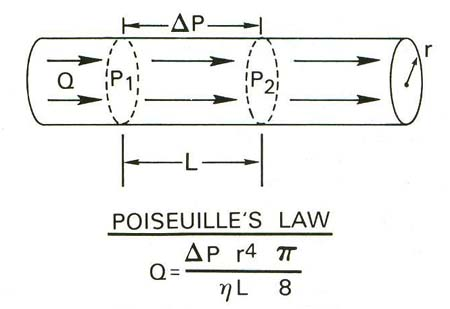
\includegraphics[width=6cm]{png/poiseuille_law.png}
 \end{center}
\end{frame}


\begin{frame}
 \frametitle{Poiseuille flow with $P_2-P_1$ elements}
 \begin{center}
 \begin{figure}
 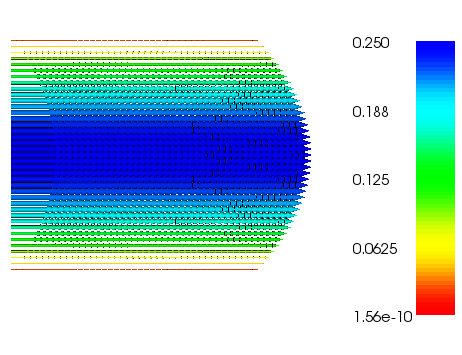
\includegraphics[width=5cm]{png/poiseuille_velocity.png}
 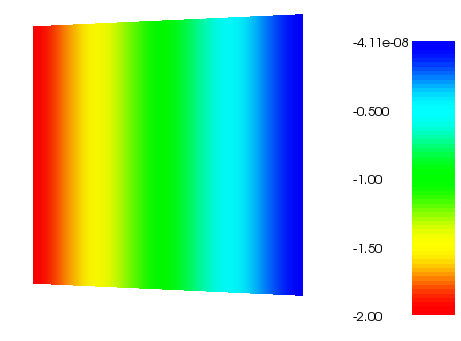
\includegraphics[width=5cm]{png/poiseuille_pressure_p2p1.png}
 \caption{Illustration of Poiseuille flow in 2D as computed with $P_2-P_1$ elements in FEniCS.
 Left image shows the velocity vectors while the right image shows the pressure.
 Both velocity and pressure are correct up to round-off error.}
 \end{figure}
 \end{center}
\end{frame}


\begin{frame}
 \frametitle{Poiseuille flow with $P_1-P_1$ elements}
 \begin{center}
 \begin{figure}
 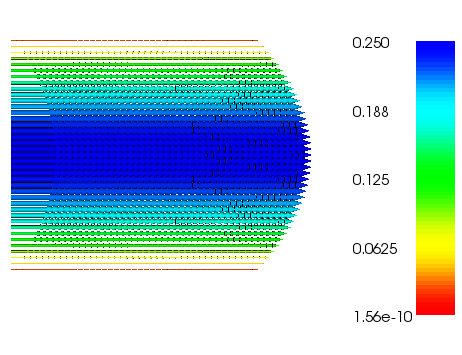
\includegraphics[width=5cm]{png/poiseuille_velocity.png}
 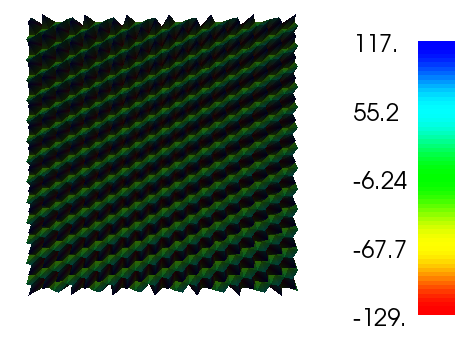
\includegraphics[width=5cm]{png/poiseuille_pressure_p1p1.png}
 \caption{Illustration of Poiseuille flow in 2D as computed with $P_1-P_1$ elements in FEniCS.
          Left image shows the velocity vectors while the right image shows the pressure.
          The velocity is correct but the pressure is \emph{not}. The $P_1-P_1$ discretization 
          violates the inf-sup condition.}
 \end{figure}
 \end{center}
\end{frame}


\begin{frame}
    \frametitle{Unstable and stable Stokes elements}
\colemph{Unstable elements} \\
        \begin{center}
            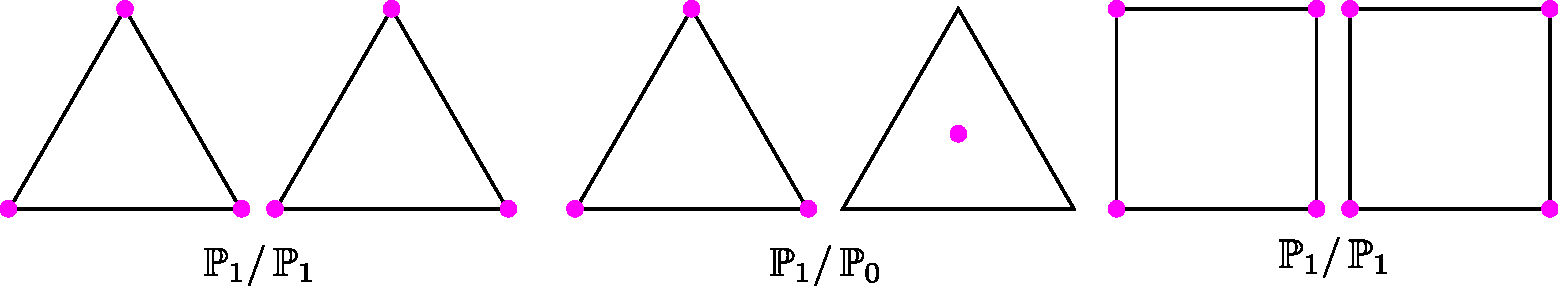
\includegraphics[width=1.0\textwidth]{pdf/stokes_unstable_elements.pdf}
        \end{center}
%    \begin{block}{Stable Stokes elements}
        \colemph{Stable elements}
        \begin{center}
            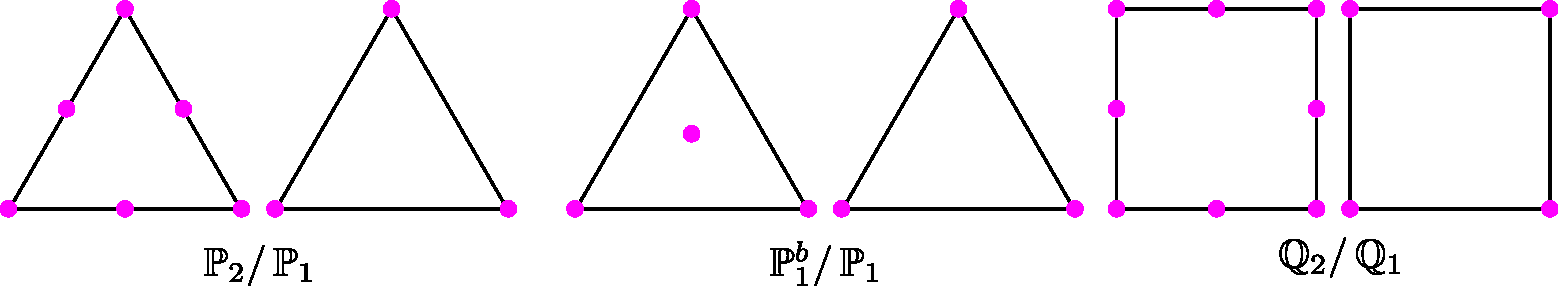
\includegraphics[width=1.0\textwidth]{pdf/stokes_stable_elements.pdf}
        \end{center}
       Taylor-Hood
        elements:  $\PP_{k+1} /\,\PP_{k}$, $\QQ_{k+1}/\,\QQ_k$ for $k\geqslant 1$  \\
        Mini-element:  $\PP_1^b/\,\PP_1$
%    \end{block}
\end{frame}



% Extra theory slides
\begin{frame}[shrink=5]
  \frametitle{The Stokes problem is a saddle point problem}
  \begin{block}{Saddle point problem}
  Given bilinear forms and linear forms
  \begin{itemize}
    \item $a(\cdot,\cdot): V\times V \to \R$
    \item $b(\cdot,\cdot): V\times Q \to \R$
    \item $L(\cdot): V \to \R$
  \end{itemize}
  Find $(u,p) \in V \times Q$
  such that
  for all  $(v,q) \in \widehat{V} \times \widehat{Q}$
  \begin{alignat}{2}
    &a(u,v) + b(v,p) & &= L(v) \nonumber
    \\
    &b(u,q) \phantom{a(u,v)} & &= 0 
  \end{alignat}
  \end{block}
  \vspace{-1em}
  \begin{block}{Operator formulation}
  Define operators (Riesz representation theorem)
  \begin{itemize}
    \item $\langle A w, v \rangle_{V',V}  = a (w,v) \qquad \foralls (w,v) \in V
      \times V$
    \item $\langle B v, q \rangle_{Q',Q}  = b (v,q) \qquad \foralls (v,q) \in V
      \times Q$
  \end{itemize}
  \vspace{-0.5em}
  \begin{alignat*}{2}
    &Au + B^{\top}p & &= L(v)
    \\
    &B u \phantom{B^{\top}} & &= 0
  \end{alignat*}
  \end{block}
\end{frame}

\begin{frame}[shrink=5]
  \frametitle{Existence, uniqueness and stability: The continuous case}
  \begin{itemize}
    \item Continuity of $A$ and $B$
      \begin{align*}
        a(w,v) \leqslant C_a \| w \|_V \|v\|_V \quad \foralls (w,v) \in
        V \times V 
        \\
        b(v,q) \leqslant C_b \| v \|_V \|q\|_Q \quad \foralls (v,q) \in
        V \times Q
      \end{align*}
 \item Coercivity of $A$ on $\Kern B$:
 \[
   c_a \| v \|_V \leqslant a(v,v) \quad \foralls v \in \Kern B 
 \]
 \item Inf-sup condition:
 \[
   \inf_{q \in Q} \sup_{v\in V} \dfrac{b(v,q)}{\|v\|_V \|q\|_Q}
   \geqslant c_b
 \]
 \item Compatibility condition for $g$
  \end{itemize}
  Then there exists a unique $(u,p) \in V\times Q$ solving
  (SPP), satisfying
  \begin{gather*}
    \| u \|_V \leqslant \dfrac{1}{c_a} 
    \| f \|_{V'} 
    \bigl(
    + \dfrac{c_a + C_a}{c_b} \|g\|_{Q^{\prime}}
    \bigr)
    \\
    \| p \|_{Q'} \leqslant \dfrac{1}{c_b}
    \bigl(
    (1 + \dfrac{C_a}{c_a}) \| f \|_{V'}
    +
    \dfrac{C_a(c_a + C_a)}{c_a c_b} \| g \|_{Q'}
    \bigr)
  \end{gather*}
\end{frame}


\begin{frame}[shrink=5]
  \frametitle{Existence, uniqueness and stability: The discrete case}
  \begin{itemize}
    \item Continuity of $A_{\alert{h}}$ and $B_{\alert{h}}$
      \begin{align*}
        a(w_{\alert{h}},v_{\alert{h}}) \leqslant C_a \| w_{\alert{h}} \|_V \|v_{\alert{h}}\|_V \quad \foralls (w_{\alert{h}},v_{\alert{h}}) \in
        V_{\alert{h}} \times V_{\alert{h}} 
        \\
        b(v_{\alert{h}},q_{\alert{h}}) \leqslant C_b \| v_{\alert{h}} \|_V \|q_{\alert{h}}\|_Q \quad \foralls (v_{\alert{h}},q_{\alert{h}}) \in
        V_{\alert{h}} \times Q_{\alert{h}}
      \end{align*}
 \item Coercivity of $A_{\alert{h}}$ on $\Kern B_{\alert{h}}$:
 \[
   c_a \| v_{\alert{h}} \|_V \leqslant a(v_{\alert{h}},v_{\alert{h}}) \quad \foralls v_{\alert{h}} \in \Kern B 
 \]
 \item Inf-sup condition: There is a \alert{mesh-independent} constant
   $c_b$ s.t.
 \[
   \inf_{q_{\alert{h}} \in Q_{\alert{h}}} \sup_{v_{\alert{h}}\in V_{\alert{h}}} \dfrac{b(v_{\alert{h}},q_{\alert{h}})}{\|v_{\alert{h}}\|_V \|q_{\alert{h}}\|_Q}
   \geqslant c_b
 \]
 \item Compatibility condition for $g$
  \end{itemize}
  Then there exists a unique $(u_h,p_h) \in V_{\alert{h}}\times Q_{\alert{h}}$ solving
  (SPP), satisfying
  \begin{gather*}
    \| u_{\alert{h}} \|_V \leqslant \dfrac{1}{c_a} 
    \| f \|_{V_{\alert{h}}'} 
    \bigl(
    + \dfrac{c_a + C_a}{c_b} \|g\|_{Q_{\alert{h}}^{\prime}}
    \bigr)
    \\
    \| p_{\alert{h}} \|_{Q_{\alert{h}}'} \leqslant \dfrac{1}{c_b}
    \bigl(
    (1 + \dfrac{C_a}{c_a}) \| f \|_{V_{\alert{h}}'}
    +
    \dfrac{C_a(c_a + C_a)}{c_a c_b} \| g \|_{Q_{\alert{h}}'}
    \bigr)
  \end{gather*}
\end{frame}


\begin{frame}
 \frametitle{The Brezzi conditions, linear algebra point of view}

Letting $u_h=\sum_{i=1}^n u_i N_i$, $p_h=\sum_{i=1}^m p_i L_i$, $v_h=N_j$, and $q_h=L_j$
we obtain a linear system on the form
\begin{equation}
\left[ 
 \begin{array}{cc}
 A & B^T\\
 B & 0
 \end{array}
\right]
\left[ 
 \begin{array}{c}
  u \\
  p 	
 \end{array}
\right]
= 
\left[ 
 \begin{array}{c}
 f \\
 0 	
\end{array}
\right]
\end{equation}
The question is what the system looks like. Two alternatives: 

\begin{tabular}[h]{lcr}
\setlength{\unitlength}{0.090in}
\begin{picture}(15,15)
\thinlines
\put(1,0){\line(0,3){3}}
\put(0.7, 0){\line(1,0){0.7}}
\put(0.7, 3){\line(1,0){0.7}}
\put(-1,1.5){$m$}
\thicklines
\put(2,0){\framebox(9,3){$B$}}

\thinlines
\put(1.9,13.6){\line(9,0){9}}
\put(1.9, 13.8){\line(0,-1){0.5}}
\put(11, 13.8){\line(0,-1){0.5}}
\put(5.5,14){$n$}
\thicklines
\put(2,4){\framebox(9,9){$A$}}

\put(12,0){\framebox(3,3){$0$}}
\put(12,4){\framebox(3,9){$B^T$}}
\end{picture}
\vspace{\unitlength}

\qquad   or \qquad

\setlength{\unitlength}{0.090in}
\begin{picture}(15,15)
\thinlines
\put(1,0){\line(0,9){9}}
\put(0.7, 0){\line(1,0){0.7}}
\put(0.7, 9){\line(1,0){0.7}}
\put(-1,4.5){$m$}
\thicklines
\put(2,0){\framebox(3,9){$B$}}

\thinlines
\put(1.9,13.6){\line(3,0){3}}
\put(1.9, 13.8){\line(0,-1){0.5}}
\put(5, 13.8){\line(0,-1){0.5}}
\put(2.5,14){$n$}
\thicklines
\put(2,10){\framebox(3,3){$A$}}

\put(6,0){\framebox(9,9){$0$}}
\put(6,10){\framebox(9,3){$B^T$}}
\end{picture}
\vspace{\unitlength}
\end{tabular}

Are both of these non-singular? How do we determine? 

\end{frame}


\begin{frame}
 \frametitle{The Brezzi conditions, linear algebra point of view, cont'd. }
 \begin{itemize}
 \item Continuity and coersivity of $A_h$ ensures that $A_h$ is non-singular 
 \item Continuity and inf-sup condition of $B_h$ ensures that $B_h$ is non-singular 
 \end{itemize}
How come we need inf-sup condition on $B_h$ ? The coersivity condition seems easier to deal with!  
\end{frame}



\begin{frame}
 \frametitle{The Brezzi conditions, linear algebra point of view, cont'd. }
 \begin{itemize}
 \item Continuity and coersivity of $A_h$ ensures that $A_h$ is non-singular 
 \item Continuity and inf-sup condition of $B_h$ ensures that $B_h$ is non-singular 
 \end{itemize}
Remember that $B_h$ is a rectangular matrix! The inf-sup condition corresponds to 
coersivity of  $B_h B_h^T$, where $B_h$ is a discrete divergence and $B_h^T$ the
discrete gradient.    

\vspace{0.3cm}
We also remark that the coersivity and inf-sup conditions are not inherited from 
the continuous operators while continuity is inherited (for conforming methods). 
\end{frame}


\begin{frame}
  \frametitle{Abstract error estimate for saddle point problems}

  \begin{align*}
    \| u - u_h \|_V 
    &\leqslant
    \bigl(
    1 + \dfrac{C_a}{c_{a,h}}
    \big)
  \inf_{v_h \in } \| u - v_h \|_V
  +
  \dfrac{C_b}{c_{a,h}}
  \inf_{q_h \in Q_h} \| p - q_h \|_Q 
  \\
  \| p - p_h \|_Q
  &\leqslant 
  \dfrac{C_a}{c_{b,h}}
  \bigl(
  1 + \dfrac{C_a}{c_{a,h}}
  \bigr)
  \inf_{v_h \in} \| u - v_h \|_V
  \\
  &\quad +
  \bigl(
  1 + \dfrac{C_b}{c_{b,h}} 
  + \dfrac{C_a C_b}{c_{a,h}c_{b,h}}
  \bigr)
  \inf_{q_h \in Q_h} \| p - q_h \|_Q
  \end{align*}

\end{frame}


\begin{frame}
\frametitle{Abstract error estimate for saddle point problems for $\PP_k-\PP_l$ discretizations}

\[
\| u - u_h \|_1 +  \| p - p_h \|_0 \leqslant C h^k \| u  \|_{k+1} +  D h^{l+1} \| p \|_{l+1}
\]


Here, $\|\cdot\|_r$ is the norm of the Sobolev space $H^r$, i.e., a
norm containing $r$ derivatives. 


Note that $k=l+1$ will give result in the simplifed estimate  

\[
\| u - u_h \|_1 +  \| p - p_h \|_0 \leqslant C h^k (\| u  \|_{k+1} + \| p \|_{k})
\]

Taylor--Hood, Crouzeix-Raviart elements are examples of such elements. 


\end{frame}


%\begin{frame}
  \frametitle{}
  \begin{columns}[T]
    \begin{column}{0.5\textwidth}
      \begin{block}{Spurious pressure nodes}
        
      \end{block}
    \end{column}
    \begin{column}{0.5\textwidth}
      \begin{block}{Degenerating inf-sup constant}
        
      \end{block}
    \end{column}
  \end{columns}
\end{frame}



% Exercises
\begin{frame}[fragile]
  \frametitle{Useful FEniCS tools (I)}
  Mixed elements:
  \vspace{-0.5cm}
  \begin{python}
V = VectorFunctionSpace(mesh, "Lagrange", 2)
Q = FunctionSpace(mesh, "Lagrange", 1)
W = V*Q
  \end{python}
 Defining functions, test and trial functions:
  \vspace{-0.5cm}
 \begin{python}
up = Function(W)
(u,p) = split(up)
 \end{python}
 Shortcut:
  \vspace{-0.5cm}
 \begin{python}
(u, p) = Functions(W)
# similar for test and trial functions
(u, p) = TrialFunctions(W)
(v, q) = TestFunctions(W)
 \end{python}
\end{frame}

\begin{frame}[fragile]
  \frametitle{Useful FEniCS tools (II)}
  Access subspaces:
  \vspace{-0.5cm}
  \begin{python}
W.sub(0) #corresponds to V
W.sub(1) #corresponds to Q
  \end{python}
 Splitting solution into components:
  \vspace{-0.5cm}
 \begin{python}
w = Function(W)
solve(a == L, w, bcs)
(u, p) = w.split()
 \end{python}
  Rectangle mesh:
 \vspace{-0.5cm}
  \begin{python}
mesh = RectangleMesh(0.0, 0.0, 5.0, 1.0, 50, 10)
  \end{python}
 \vspace{-0.5cm}
  \begin{python}
h = CellSize(mesh)
  \end{python}
%  Defining $\Delta$:
% \vspace{-0.5cm}
%  \begin{python}
%div(grad(u)) # as expected :)
%  \end{python}
\end{frame}

%\fenicssection{Demo: Couette flow}
%\fenicssection{Demo: Taylor--Hood elements}
%\begin{frame}
    \frametitle{Spurious pressure modes}
    \begin{block}{What can go wrong?}
        \colemph{Spurious pressure modes} occur if
        $\Kern B_h^T \not\subset  \Kern B^{\top}$.
        \\
        \vspace{1em}
        \colemph{Degeneration of the inf-sup constant:}
        $c_b = c_b(h)$ and $c_b(h) \rightarrow 0, h \rightarrow 0$.
%        \uncover<2->{
%        Note that $c_b$ does only appear in the \apriori{} estimate for
%        $\| p - p_h \|$ $\Rightarrow$ unstable element can give
%        good approximations for $u$ but useless approximations for $p$.
%    }
    \end{block}
%    \vspace{-1em}
    \begin{block}{Exercise: Couette flow}
        Compute the finite element approximation for Couette
        flow on the unit square. Use the boundary data
        \begin{equation*}
            u = 1  \text{ on } y = 1, \quad
            u = 0  \text{ on } y = 0, \quad
          g_N = 0  \text{ on } x = 0 \text{ or } x = 1
        \end{equation*}
%        \begin{center}
%            \includegraphics[width=0.5\textwidth]{}
%        \end{center}
        Use $\PP_1 /\,\PP_1$ and $\PP_1 /\, \PP_0$
        elements. The exact solution is given by
        \[
            u = (y,0), \qquad p = 0
        \]
        What do you observe? Why?
    \end{block}
\end{frame}


%\begin{frame}
    \frametitle{Exercise: Spurious pressure modes}

    Compute the finite element approximation for Couette
    flow on the unit square. Use the boundary data
    \begin{equation*}
      u = 1  \text{ on } y = 1, \quad
      u = 0  \text{ on } y = 0, \quad
      g_N = 0  \text{ on } x = 0 \text{ or } x = 1
    \end{equation*}
    %        \begin{center}
%            \includegraphics[width=0.5\textwidth]{}
%        \end{center}
    Use $\PP_1 /\,\PP_1$ and $\PP_1 /\, \PP_0$
    elements. The exact solution is given by
    \[
    u = (y,0), \qquad p = 0
    \]
    What do you observe? Why?
\end{frame}


%\begin{frame}
    \frametitle{Exercise: A stabilized $\PP_1/\,\PP_1$ method}
    Define  the bilinear forms
    \begin{align*}
        a_h(u_h,v_h) &= (\nabla u_h, \nabla v_h)  \\
        b_h(v_h,q_h) &= -(\nabla \cdot v_h, q_h)  \\
        c_h(p_h,q_h) &= \sum_{T \in \mesh_h}\mu_T(\nabla p_h, \nabla
        q_h)
    \end{align*}
%    \vspace{-1em}
    and solve: find $(u_h,p_h) \in V_h \times Q_h$
    such that $\foralls (v_h,q_h) \in \widehat{V}_h \times \widehat{Q}_h$
    \begin{align*}
        A(u_h,p_h;v_h,q_h) &:= a(u_h,v_h) + b(v_h,p_h) + b(u_h,q_h) -
        c(p_h,q_h)
        \\
        &= (f,v_h) - \sum_{T \in \mesh_h}\mu_T (f,\nabla q_h)
    \end{align*}
    \colemph{Exercise:}
    Implement this scheme for the Couette flow example using
    $\mu_T = \beta h_T^2$, $\beta = 0.2$.
    %How is this scheme related to the stabilized
    %$\PP_2 /\, \PP_2$ elements introduced in the second lecture today?
\end{frame}


%\fenicssection{Demo: Stabilized elements}

% Extra slides
\begin{frame}[shrink=10]
    \frametitle{The FEniCS challenge!}
    \vspace{1em}
    \begin{columns}[c]
        \begin{column}{0.5\textwidth}
            Compute the Stokes flow around a swimming dolphin!
            \begin{itemize}
                \item Set a no-slip boundary condition on the upper and
                    lower channel walls and around the dolphin
                \item Set $u = (-\sin(\pi y),0)$ on the right inflow
                    boundary
                \item Impose $p=0$ on the left outflow boundary
                \item Implement a scheme based on Taylor--Hood elements
                \item Implement a scheme based on the stabilized
                $\PP_2/\,\PP_2$ elements with a stabilization parameter
                    $\beta$.  What happens if you reduce the size of
                    $\beta$?
            \end{itemize}
        \end{column}
        \begin{column}{0.5\textwidth}
            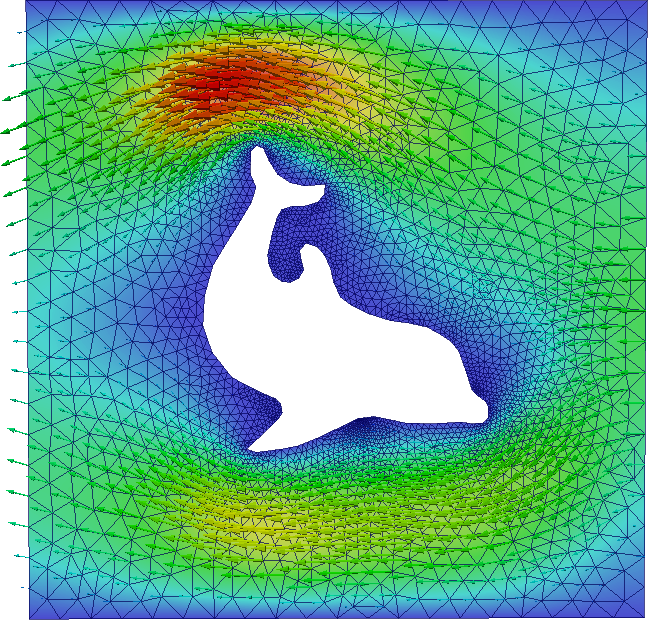
\includegraphics[width=1.0\textwidth]{png/stokes_dolphin_channel_u_alpha.png}
        \end{column}
    \end{columns}
    \begin{center}
    \end{center}
\end{frame}

\begin{frame}
\frametitle{Exercise: check the convergence of a known scheme}

We had the error estimate: 
\[
\| u - u_h \|_1 +  \| p - p_h \|_0 \leqslant C h^k \| u  \|_{k+1} +  D h^{l+1} \| p \|_{l+1}
\]
Check if this is correct by manufacturing a right-hand side (and bc) 
from a known solution. 
Assume that $u=\nabla\times sin(\pi x y)$ 
and $p= sin(2\pi x)$ and compute the right-hand side
as $f=-\Delta u + \nabla p$. 
The $\nabla\times$ operator is defined as $(-\frac{\partial}{\partial y}, \frac{\partial}{\partial x})$.
Compute numerical solutions
$u_h$ and $p_h$ on refinements of the unit square and check 
it the error estimate is valid. Use Taylor-Hood ($\PP_2-\PP_1$) 
as well as ($\PP_1-\PP_1$).   

\end{frame}

%\input{slides/stokes_couette_flow}
%\input{slides/stokes_fenics_3}
%\begin{frame}
    \frametitle{Warm-up exercise}
    \begin{center}
        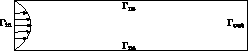
\includegraphics[width=0.9\textwidth]{pdf/channel.pdf}
    \end{center}
    Implement a solver for Hagen--Poiseuille flow
    (parabolic flow profile) in a 2D channel based on the
    $\PP_2/\,\PP_1$ Taylor-Hood element. Assume that
    \begin{itemize}
        \item the channel is of length $l = 5$ and height $h = 1$
        \item $v_{\text{max}} = 1$
        \item an inflow boundary condition is given on
            $\Gamma_{\text{in}}$
        \item a no-slip boundary condition is given at the channel
            walls $\Gamma_{\text{out}}$.
        \item a ``do-nothing'' boundary condition ($g_N = 0$) is imposed on the
            outflow boundary $\Gamma_{\text{out}}$
    \end{itemize}
\end{frame}

%\input{slides/stokes_error_estimate}
%\input{slides/stokes_stabilized_method_example}
%\input{slides/stokes_homework_2}

\end{document}
